\documentclass[twocolumn,10pt]{article}
\usepackage[a4paper, top=1.0in, bottom=1.0in, left=0.85in, right=0.85in]{geometry}

\usepackage{graphicx}
\usepackage{algorithm}  
\usepackage{algorithmicx}  
\usepackage{algpseudocode}  
\usepackage{amsmath}
\usepackage{url}
\usepackage{xcolor}
\usepackage{listings}

\renewcommand{\algorithmicrequire}{\textbf{Input:}}  
\renewcommand{\algorithmicensure}{\textbf{Output:}}  
\graphicspath{{figure/}}

\lstdefinelanguage{swift}
{
	morekeywords={
		func,if,then,else,for,in,while,do,switch,case,default,where,break,continue,fallthrough,return,
		typealias,struct,class,enum,protocol,var,func,let,get,set,willSet,didSet,inout,init,deinit,extension,
		subscript,prefix,operator,infix,postfix,precedence,associativity,left,right,none,convenience,dynamic,
		final,lazy,mutating,nonmutating,optional,override,required,static,unowned,safe,weak,internal,
		private,public,is,as,self,unsafe,dynamicType,true,false,nil,Type,Protocol,
	},
	morecomment=[l]{//}, % l is for line comment
	morecomment=[s]{/*}{*/}, % s is for start and end delimiter
	morestring=[b]" % defines that strings are enclosed in double quotes
}
\definecolor{keyword}{HTML}{BA2CA3}
\definecolor{string}{HTML}{D12F1B}
\definecolor{comment}{HTML}{008400}
\lstset{
	language=swift,
	basicstyle=\ttfamily,
	showstringspaces=false, % lets spaces in strings appear as real spaces
	columns=fixed,
	keepspaces=true,
	keywordstyle=\color{keyword},
	stringstyle=\color{string},
	commentstyle=\color{comment},
}

\begin{document}
\small
\date{July 11th, 2017}

\title{\bf Grouper: a Framework for Developing Mobile Application using Secret Sharing and Untrusted Servers}

\author{
	Meng Li, 201620728  
	\\ Supervisor: Yasushi Shinjo
}

\maketitle

\section{Introduction}
Conventional client-server mode applications requires central servers for storing shared data. The users of such mobile applications must fully trust the central server and their application providers. If central servers are compromised by hackers, user information may be revealed because data is often stored on the server in cleartext. Users may lose their data when service providers shut down their services. 

To address these problems, Grouper use multiple untrusted servers for data transfer. Data is divided into several pieces by the Secret Sharing scheme and uploaded to diverse servers. Each server can only keep a piece of data temporarily, we call it share. A share will be deleted after a period of time. These ensure that user data cannot be cracked easily. In addition, all devices of group members keep a complete data set, and data can be recovered even untrusted servers shut down.

\section{Design}
We design this framework on the iOS platform at first. We are aiming at developing applications which are not relying on trusted central servers. Applications based on Grouper can synchronize data among group members' devices. Each group member holds one device. In this sections, we introduce some important concepts in Grouper.

\subsection{Secret Sharing}
In Grouper, a device uses a Secret Sharing scheme to divide a message into several shares and upload them to multiple untrusted servers. Other devices download shares and recover the original message by Secret Sharing scheme. In a Secret Sharing scheme, a member securely shares a secret with a group of members by generating $n$ shares using a cryptographic function\cite{smith2013layered}. At least $k$ or more shares can reconstruct the secret, but $k-1$ or fewer shares can obtain nothing about the secret\cite{pang2005new}. We describe this scheme as a function $f(k, n)$, where $n$ is the number of all shares, and $k$ is the threshold to combine shares. 

\subsection{Multiple Untrusted Servers}

Unlike central trusted servers, we design Grouper based on data synchronization through multiple untrusted servers. There are some principles in our proposal. 

Firstly, a server transfers data as similar to a router, and does not keep it permanently. Most current popular client-server applications store their user data on several central servers, and the user's data will not be deleted unless the user deletes his account. Grouper uses untrusted servers as a bridge for transferring data.

Secondly, a server keeps data temporarily. We define a period of time in which data can be kept in a server, we call it interval time. The record a sender uploaded to untrusted servers can exist within the interval time. After the interval time, this record will be deleted.

Thirdly, servers do not know the cleartext of data. Keeping data temporarily cannot ensure data security, because servers know the cleartext of data in this temporary period. For this problem, developers often encrypt data before uploading to servers, and this needs a decryption key to decrypt data in other devices. In Grouper, we use a Secret Sharing scheme as described in section 2.1 rather than data encryption. Servers do not know the cleartext of a share generated by the Secret Sharing scheme.

\subsection{Data Synchronization}

\begin{figure}[!htb]
	\centering
	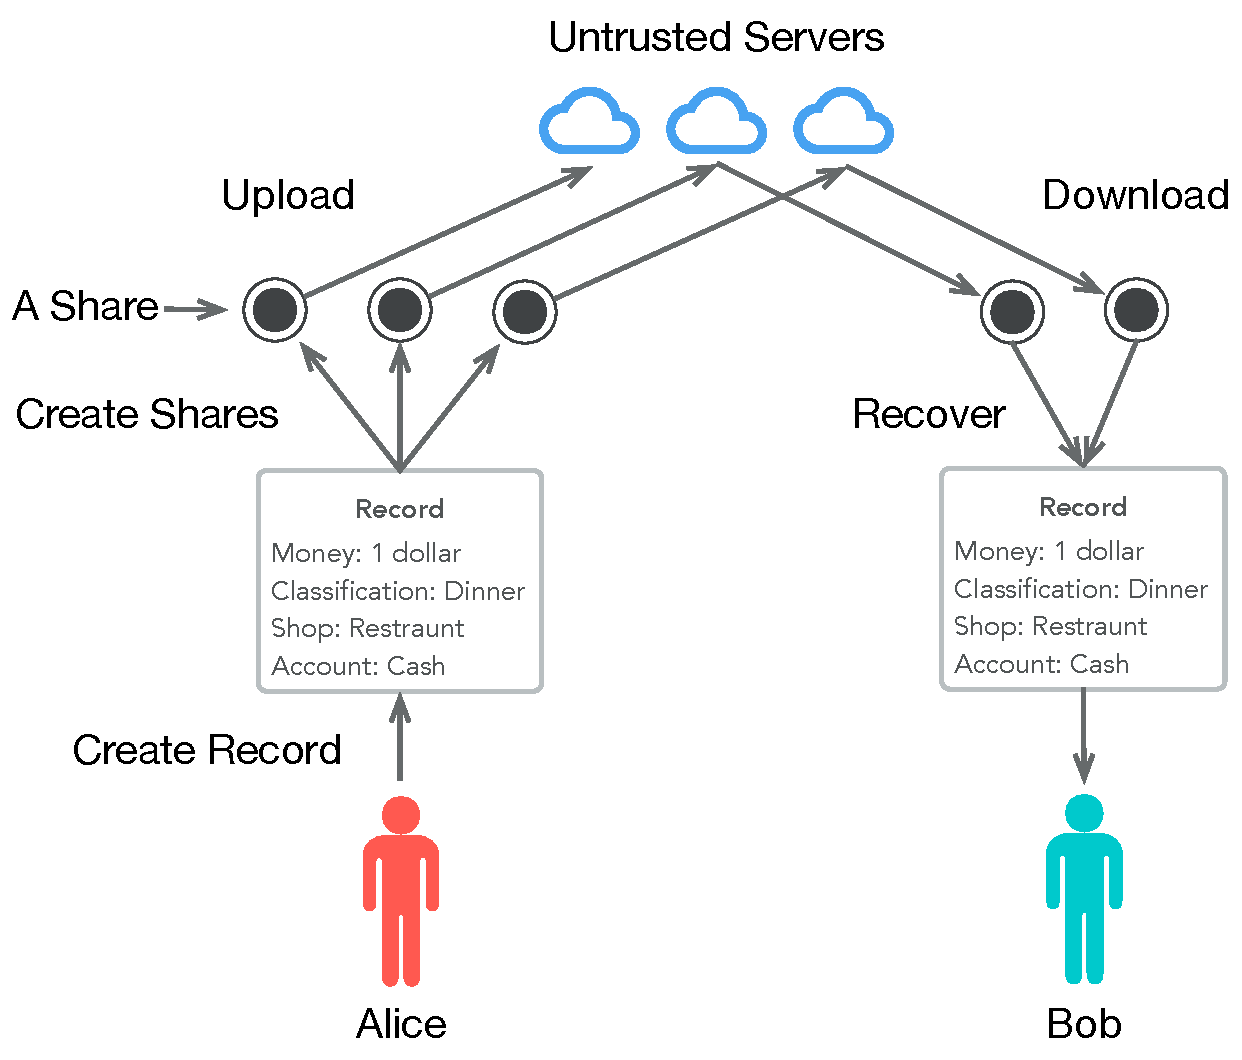
\includegraphics[scale=0.38]{sync_flow}
	\caption{Data Transportation Flow}
\end{figure}

Figure 1 describes our data transportation flow based on the principles described in section 2.2. At first, the sender adds a record and Grouper creates three shares by a secret sharing scheme where $n$ is three and $k$ is two. Next, Grouper uploads those shares to three untrusted servers. When the receiver is online, he downloads two shares from two servers and recovers the new record. In this process, each server is separated from other servers, and cannot access to other servers. This means these servers cannot recover user data because they do not have permission to access other untrusted servers. In our proposal, only group members have permission to access these untrusted servers.

\subsection{Reliable Synchronization}
Grouper should provide a reliable synchronization service. A user in a group creates a new record and all of other members in this group should synchronize this record, even if this record may be deleted by untrusted servers after a interval time. We call this problem reliable synchronization. A receiver can only download shares from untrusted server with the interval time. If he synchronize data after the interval time, he will miss the new record from the sender.

\begin{figure}[!htb]
	\centering
	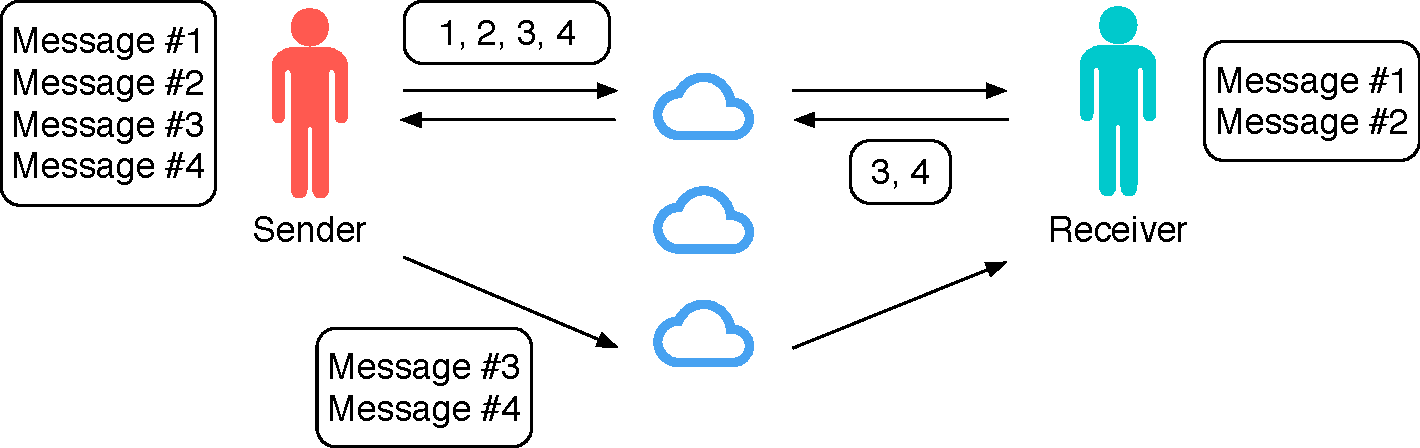
\includegraphics[scale=0.3]{reliable_sync}
	\caption{Reliable Synchronization}
\end{figure}

To solve this problem, we use the idea of reliable multicasting in distribute systems. In Figure 2, the sender has sent messages from No.1 to No.4. Next, he sends sequence numbers of all messages he sent to the receiver. When the receiver receives the sequence numbers, he will check his local persistent store. In this situation, the receiver will find that he missed the message No.3 and No.4. Thus, he will send a request that contains the sequence numbers of messages he missed to the sender. At last, the sender will resend the message No.3 and No.4 to the receiver again.

\subsection{Grouper Message}

To transfer data between devices, we design our own \emph{Grouper Message}. A Grouper message is a JSON string that contains the entities of the application and the way to handle it in receivers’ devices. There are 4 types of Grouper messages: update message, delete message, confirm message and resend message. Both update message and delete message need resend because they contain entities of the application. We call them normal messages. Both confirm message and resend message contain control information about reliable multicast and need not resend. We call them control messages.

When a user creates a new entity or modifies some attributes of an existing entity, the device sends an update message that contains the JSON string of this entity to all group members.

When a user deletes an existing entity, the device sends a delete message that contains the object ID of this entity to all group members.

To confirm all group members have received all normal messages created by a user, the device of him need to send confirm message to group members periodically. In Grouper, when the application is launched, it should check the last send time of confirm message. If the last confirm message is sent within interval time, the device need not to send a confirm message again. Otherwise, the devices need to send a new confirm message contains the sequences of all normal messages created by this user before.

When the device of a group member receives a confirm message, it should check the sequences. If some of them does not exist in its' persistent store, the device sends a resend message that contains sequence numbers that are not in the persistent store.

\subsection{Group Management}

\subsubsection{Creating a Group}

A group is created by its owner. Before creating a group, the owner prepares his own user information including his email and name, multiple untrusted servers, a group ID and a group name. For example, Alice assigns the group ID and group name and registers them to all untrusted servers of this group. Next, she initializes this group on all untrusted server by submitting her node identifier. The node identifier, which represents her device, is generated by Grouper framework randomly when the application is launched at first the time. In each untrusted server, the Web service initializes this new group and returns a master key including the highest privilege to the owner. The owner can add other members to an untrusted server by the master key.

\subsubsection{Inviting a Member}

After creating a group, the owner can invite a new member to his group. To join the group, the new member prepares his user information at first. The owner invites the new member by a face-to-face way rather than using central servers. Before inviting, Grouper establishes connection between their devices. Firstly, the new member sends user information and a node identifier to the owner. Owner saves user information and the node identifier of the new member to his device. Secondly, the owner register the new member on multiple untrusted servers by submitting the node identifier of the new member. Thirdly, untrusted servers returns access keys for the new member to the owner. Lastly, the owner sends the access keys, server addresses and existing members' list to the new member. After receiving them, the new member can access untrusted servers.

\section{Implementation}

Grouper consists of a client framework for developing iOS application and a Web service running on multiple untrusted servers. In Section 2, we have introduced how to share strings with other deices via multiple untrusted servers. In this section, we describe persistent store and data synchronization. Grouper stores all data on mobile devices with an object-oriented way.

\subsection{Web Service}
Grouper needs its own Web service rather than using commercial general cloud services like Amazon S3, Google Cloud for following reasons:

\begin{itemize}
	\setlength{\itemsep}{1pt}
	\setlength{\parskip}{0pt}
	\setlength{\parsep}{0pt}
	\item The Web service supports reliable synchronization.
	\item The Web service ensures that shares are deleted after a prescriptive time.
\end{itemize}

Our web service provides RESTful API to transfer data with clients, and it keeps shares from devices temporarily. It runs on the Tomcat server that is an open source implementation of the Java Servlet, JavaServer Pages, Java Expression Language and Java WebSocket technologies. We use the Spring MVC, a  Web model-view-controller framework, to create our RESTful API, and Hibernate, an open source Java ORM framework, to save and operate objects in the Web service. 

Our Web service includes three entities. They are \emph{Group}, \emph{User} and \emph{Transfer}. A \emph{Group} entity saves a group ID, a group name and its owner. A \emph{User} entity saves the node identifier of a user, the access key for this user, and group of this user. A \emph{Transfer} entity saves a share generated with a secret sharing scheme, the time when the user uploads it and its creator. For each user, there is a unique access key for him in an untrusted server. For a group, one of a user is its owner who has the highest privilege of this group.

\subsection{Client}

Grouper provides a client framework by Objective-C language to developing applications on iOS, macOS, watchOS and tvOS. Figure 3 describes the architecture of client framework. It is based on such frameworks.   

\begin{figure}[!htb]
	\centering
	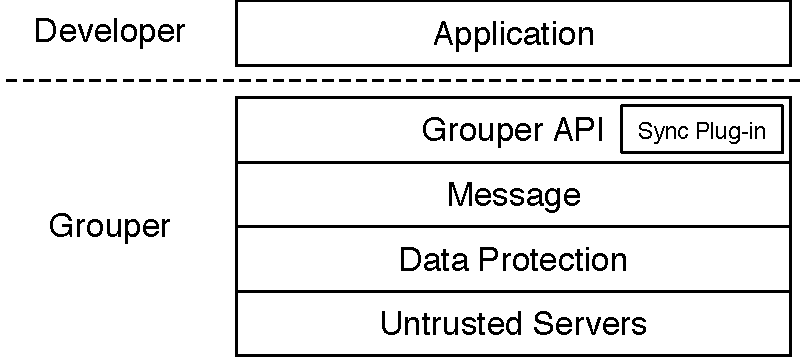
\includegraphics[scale=0.35]{architecture}
	\caption{Architecture of Client}
\end{figure}

\begin{itemize}
	\setlength{\itemsep}{1pt}
	\setlength{\parskip}{0pt}
	\setlength{\parsep}{0pt}
	\item Grouper used \emph{Multipeer Connectivity}\cite{mc},  a official peer-to-peer communication framework provided by Apple, to transfer data between devices by a face-to-face way.
	\item Grouper uses \emph{Core Data}\cite{coredata}, a official ORM framework provided by Apple, to manage the model layer objects.\emph{Core Data} provides generalized and automated solutions to common tasks associated with object life cycle and object graph management, including persistence.
	\item Grouper uses \emph{Sync}\cite{sync}, a modern JSON synchronization framework for \emph{Core Data}, to create JSON strings and synchronize object from JSON strings.
	\item Grouper uses \emph{c-SSS}\cite{c-sss}, an implementation of Shamir's secret sharing in the C language, to create shares and recover shares.
	\item Grouper uses \emph{AFNetworking}\cite{afnetworking}, a delightful networking library by Objective-C language, to revoke the RESTful API provided by our Web services. 
\end{itemize}

With {Core Data} and {Sync}, Grouper can synchronize data to persistent store.

\section{Demo}
Using Grouper framework, we have developed an iOS app \emph{Account Book} that can record the income and expenditure, in Objective-C language, and an benchmark iOS app \emph{Test} in Swift language to test the performance of Grouper. We are developing a macOS app \emph{Notes} that can take notes for small group in Swift language.

\section{Evaluation}

This section answers two main questions:  first, how much developer effort is required to use Grouper, and second, what are the performance overheads of Grouper?

\subsection{Developer Effort}

There are two factors that will influence the developer effort: the usability of client API and the lines of code(LoC) the developer has to add.

\begin{description}
	\item[Client API] Grouper provides very simple client API for developers.
\end{description}

\begin{lstlisting}
// Initialize Grouper
grouper.setup(withAppId:"test",
dataStack:DataStack(modelName: "test")) 
// Create Object & Update Object
grouper.sender.update(test)
// Delete Object
grouper.sender.delete(test)
// Receive Object
grouper.receiver.receive { 
// Callback after receiving objects.
}
//Send Confirm Message
grouper.sender.confirm()
\end{lstlisting}

\begin{description}
	\item[LoC] We developed 2 applications including \emph{Account Book} and \emph{Test} with Grouper. As described in table 1, compared with application LoC, Grouper related LoC that developer has to add is only a small part. 
\end{description}

\begin{table}[!htb]
	\centering
	\caption{Demo app's lines of code}
	\label{my-label}
	\begin{tabular}{c|c|c}
		\hline
		Attribute           & Test  & Account Book \\ \hline
		Platform            & iOS   & iOS          \\ \hline
		Lanaguage           & Swift & Objective-C  \\ \hline
		Application LoC     & 632   & 8950         \\ \hline
		Grouper related LoC & 11    & 19           \\ \hline
		Number of Entities  & 1     & 5            \\ \hline
	\end{tabular}
\end{table}

\subsection{Performance}

The performance goal is to avoid significantly affecting the user experience with the application developed with Grouper. To evaluate whether Grouper meets this goal, we use the benchmark app \emph{Test} with the $f(2, 3)$ Secret Sharing scheme to transfer data between iPhone 4s and iPod 5 generation on LAN network. We answer the following questions about performance:

\begin{figure}[!htb]
	\centering
	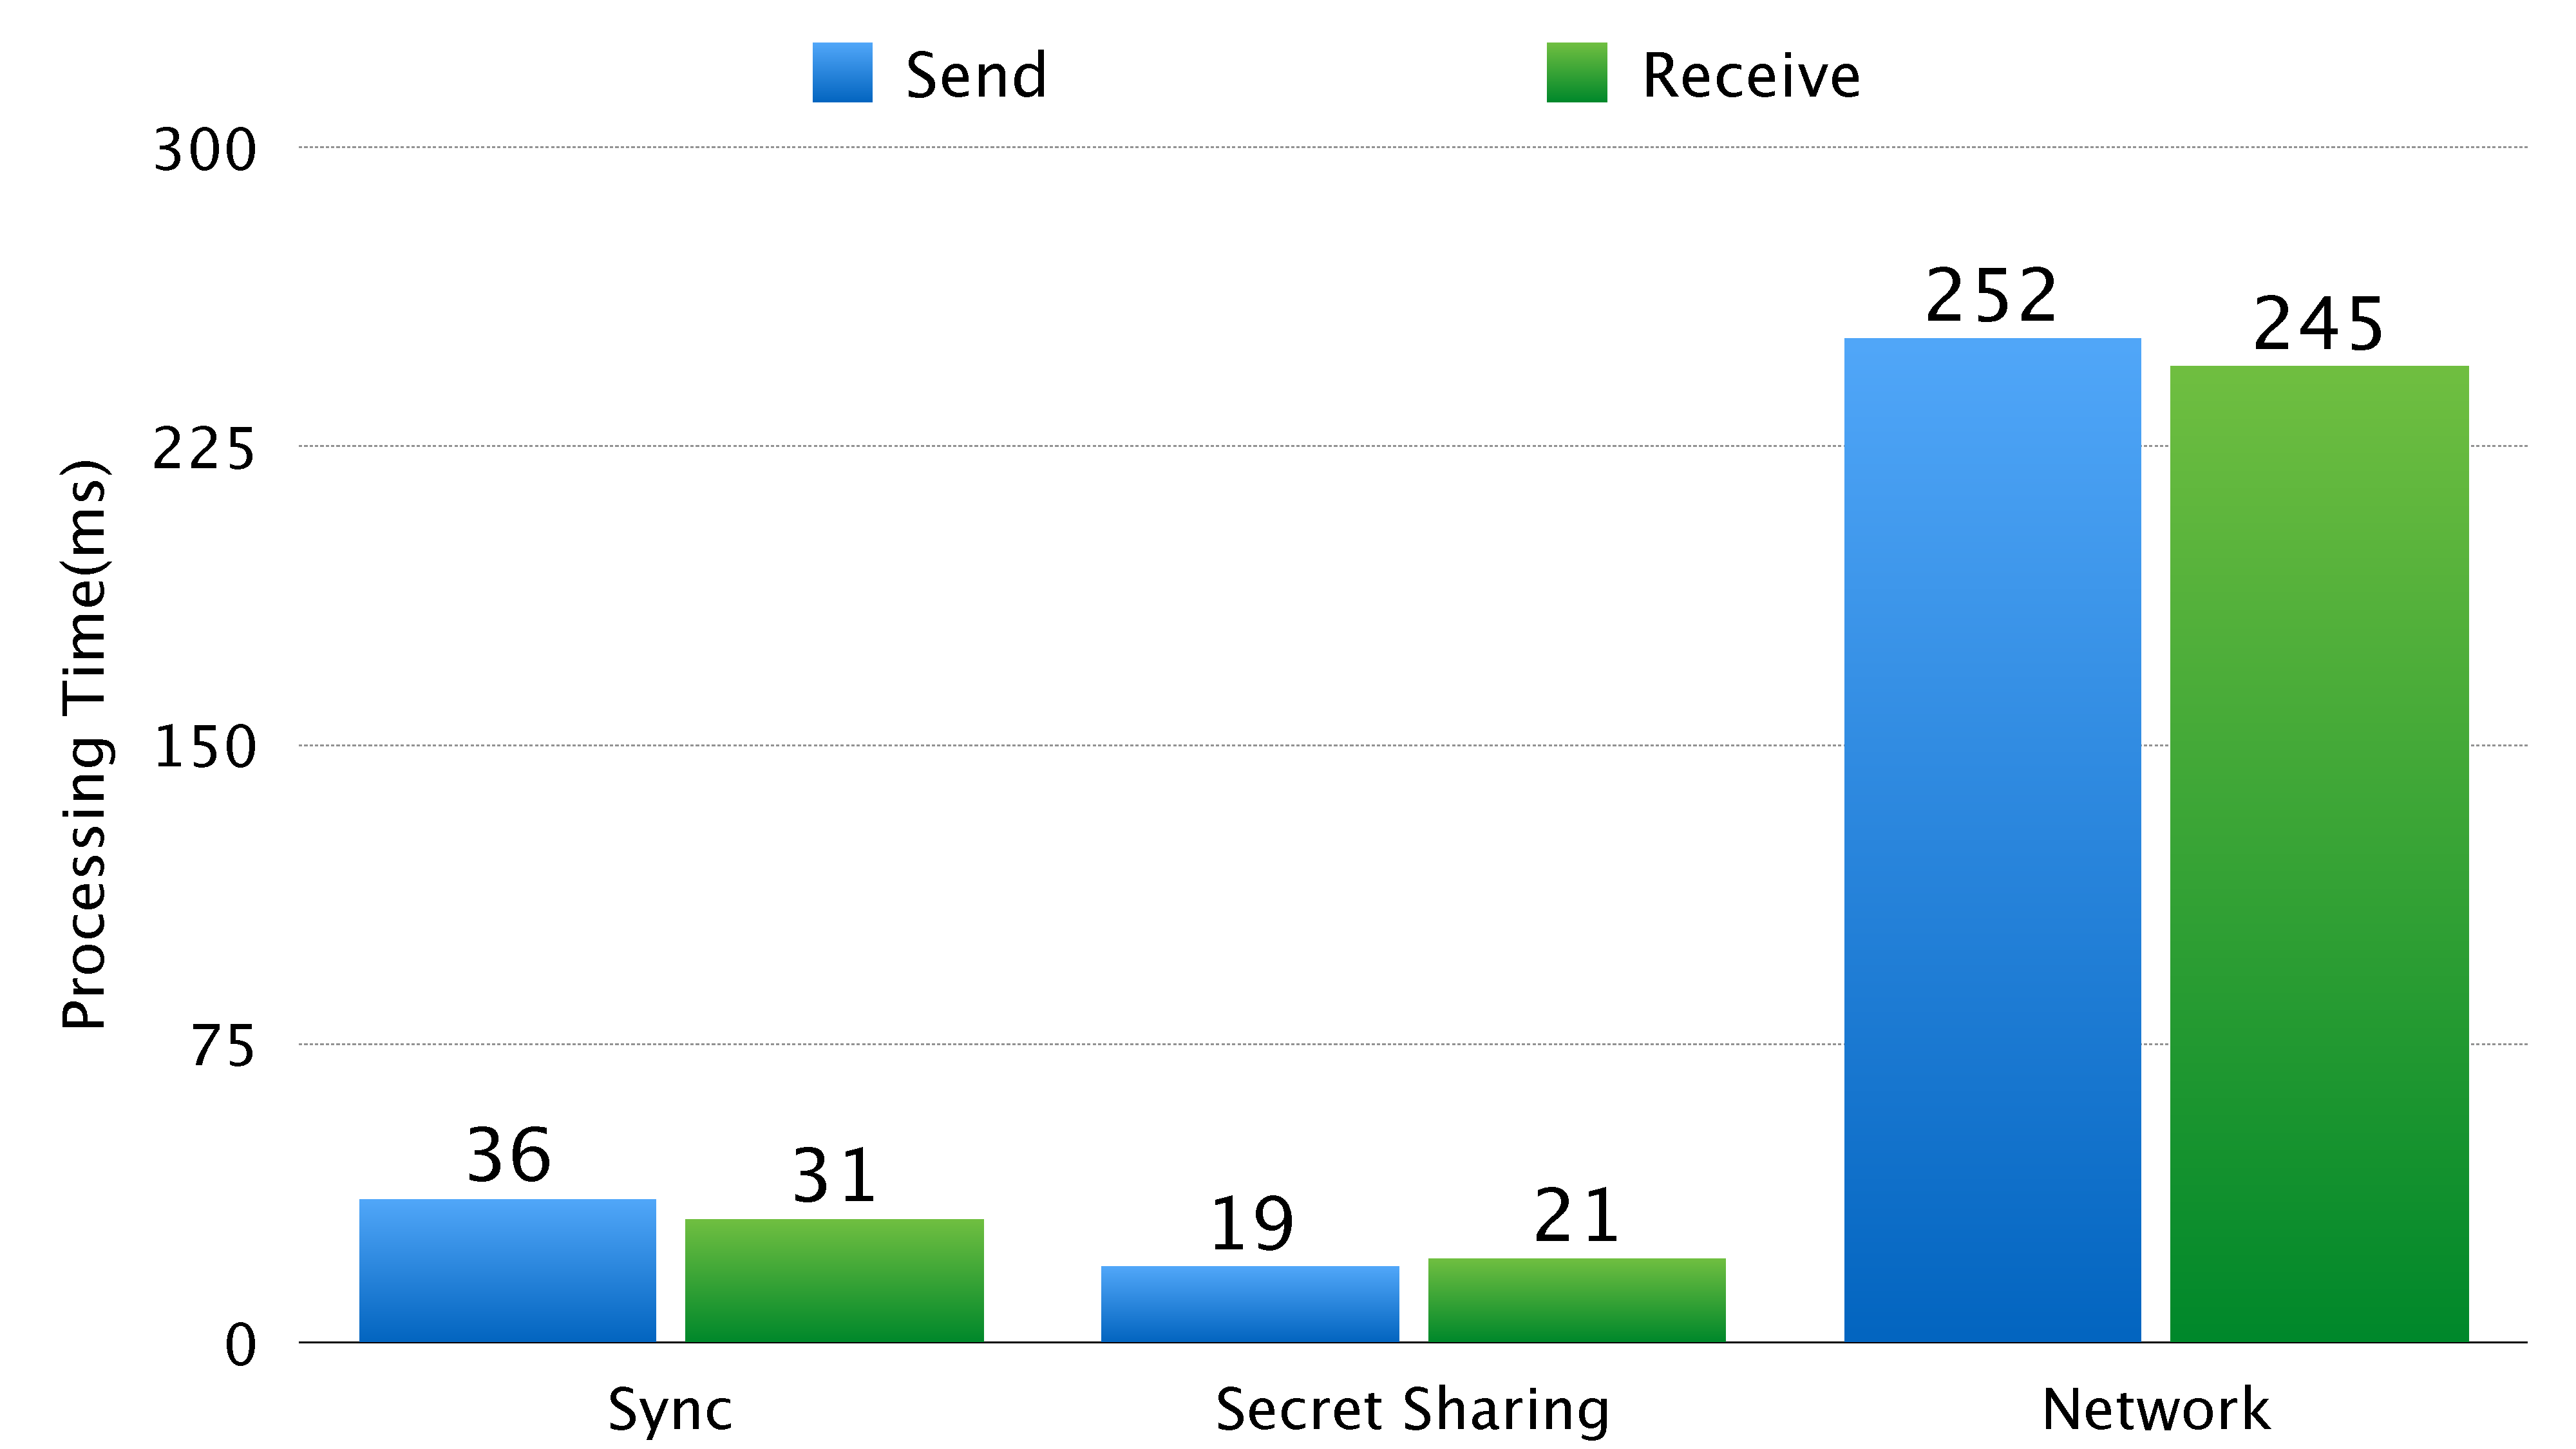
\includegraphics[scale=0.12]{processing1}
	\caption{Sending and Receiving 1 Message}
\end{figure}

\begin{figure}[!htb]
	\centering
	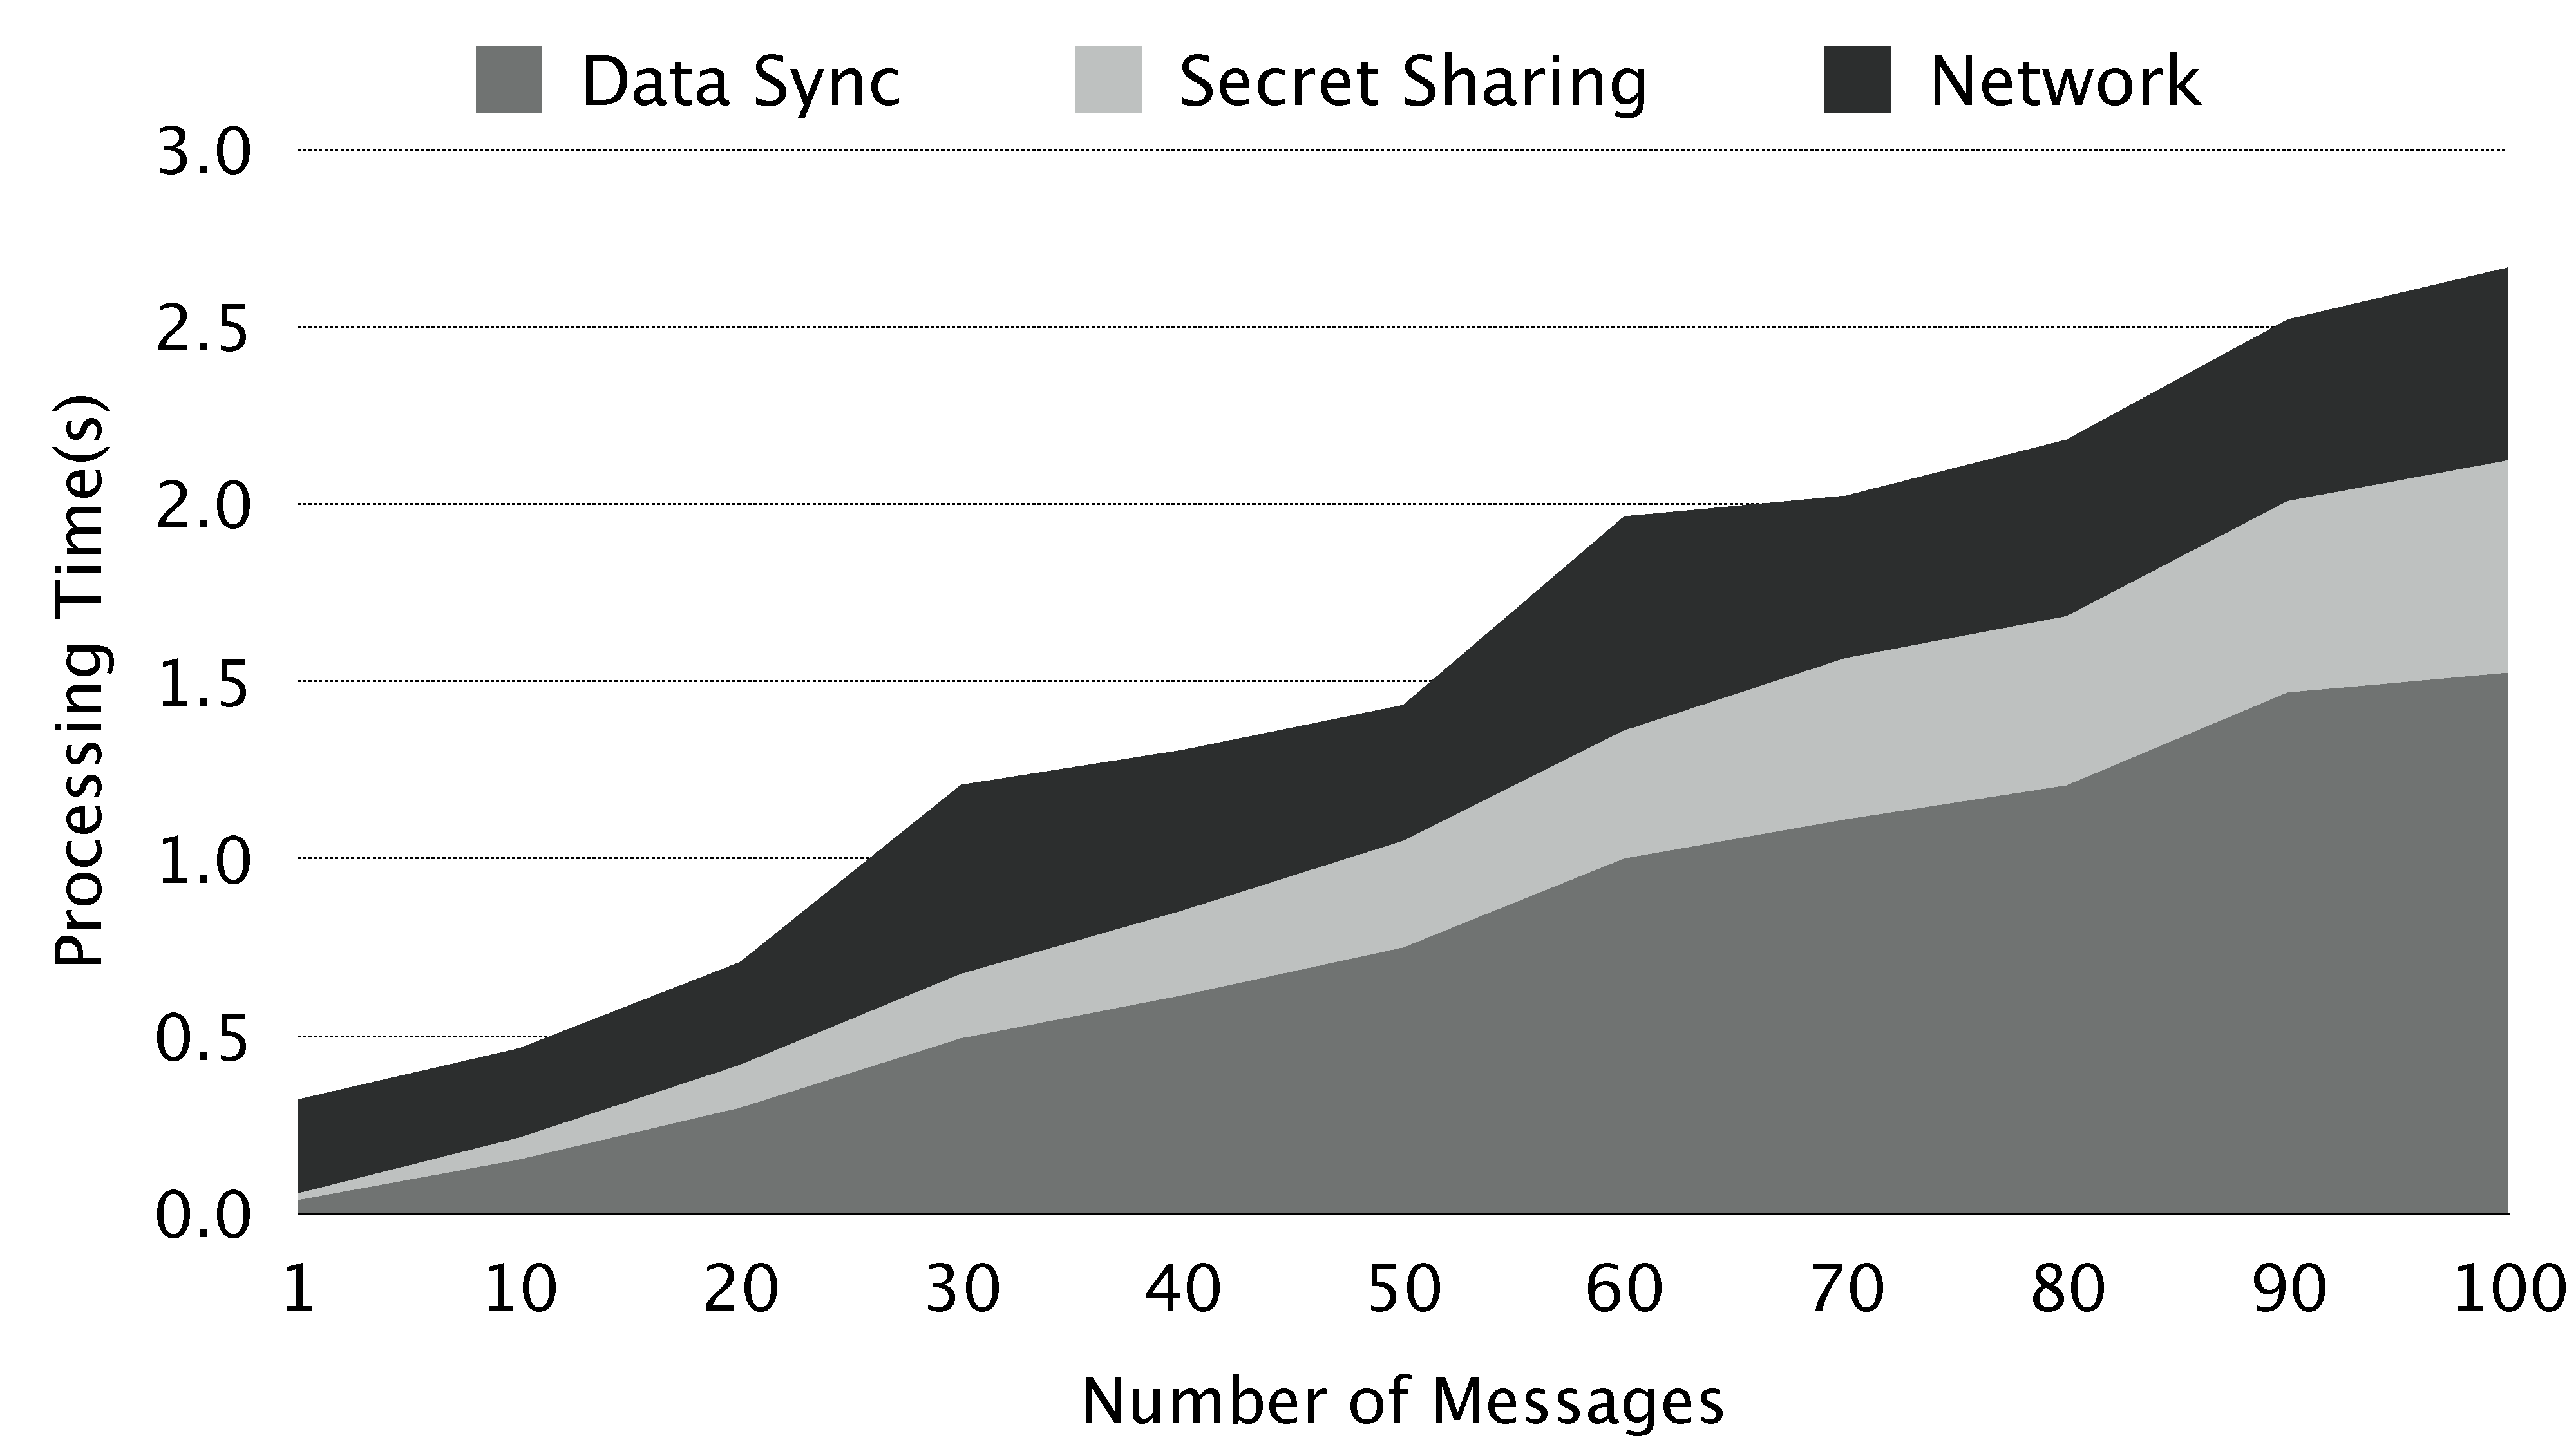
\includegraphics[scale=0.12]{processing2}
	\caption{Sending Multiple Messages}
\end{figure}

\begin{description}
	\item[Data Sending:] How much processing time does Grouper add to app when a user creates objects?
	Figure 4 shows the processing time for sending and receiving 1 message. Compared to network, data sync and secret sharing consume very little time in both data sending and receiving.
	\item[Data Sending:] How much processing time does Grouper add to app when a user wants to synchronize data from untrusted servers?
	Figure 5 shows the processing time for sending multiple messages. With the increasing of messages number, data sync and Secret sharing part increase linearly. The network part increases very slowly and sometimes decrease.
\end{description}

\section{Related Work}

To solve this problem, some applications use Peer to Peer(P2P) to transfer user data between devices. Some applications encrypt and decrypted user data in clients and save encrypted data in servers. 

Mylar\cite{popa2014building} stores encrypted and sensitive data on a server, and decrypts this data only in users’ browsers. Developers of Mylar use its API to encrypt a regular(non-encrypted) Web application, and users decrypt data by a browser extension. Like in Grouper, applications in Mylar can control how user data is shared and store data on multiple untrusted servers. Mylar builds its system on a browser with extension while Grouper uses mobile devices.

Sweets\cite{sweets} is a decentralized social networking service mobile application using data synchronization with P2P connections between devices. Sweets use AES(Advanced Encryption Standard) scheme to encrypt user data and ABE(Attribute Based Encryption) scheme to encrypt the key of AES. However, there is an obvious problem in such a P2P approach. Data transfer can only be finished during two devices are online at the same time. Thus, Grouper uses multiple untrusted servers to synchronize user data rather than P2P in Sweets.

\section{Future Work and Conclusion}

In the future, we will concentrate on such works:
\begin{itemize}
	\setlength{\itemsep}{1pt}
	\setlength{\parskip}{0pt}
	\setlength{\parsep}{0pt}
	\item Finish the demo application \emph{Notes} on macOS,
	\item Solve the synchronization order and JSON string redundancy caused by One-To-Many entity relationship.
	\item Improve the performance by retaining only 1 normal message for 1 object in untrusted servers .
\end{itemize}

This paper introduces Grouper, a framework Secret sharing and multiple untrusted server, to develop applications which is not relying on trusted central server. Grouper provides two main functions: reliable data synchronization and group management. We implement Web service by Java EE and client framework by Objective-C language. We use Grouper to develop demo applications including \emph{Account Book}, \emph{Notes} and \emph{Test}. At last, we evaluate Grouper from developer effort and performance.

\bibliographystyle{unsrt}
{
	\footnotesize
	\bibliography{ref}
}

\end{document}
